\documentclass[a4paper,11pt,spanish,twoside]{article}

\usepackage{mteoptions}
\usepackage{mtereport}
\usepackage{wrapfig}
\usepackage{multicol}

\lstset{basicstyle=\footnotesize}

\begin{document}
\title{Practica:  Caracterización de la workload de CPU}

\author{Miguel Tellería }

\date{6 Marzo 2012}

\maketitle
\thispagestyle{empty} % no page number in the first page

% -----------------------------------------------------------------------------
% ABSTRACT
% -----------------------------------------------------------------------------
\begin{abstract}

El objetivo de la práctica es familiarizarse con diferentes tipos de
workloads de CPU y ser capaz de estimar a partir de una ejecución de
CPU métricas de ocupación y utilización de la CPU.

\end{abstract}

\section{Objetivo}
\label{sec:objetivo}

Dada una configuración de nuestro programa de cargas sintéticas, ser
capaz de:

\begin{itemize}
\item Generar una captura de uso de CPU con ftrace/trace-cmd/kernelshark.

\item Extraer de los datos de dicha captura muestras para sacar
  perfiles estadísticos.

\end{itemize}

\section{Trabajo a realizar}
\label{sec:trabajo}

\subsection{Ejecución y captura de cargas}
\label{sec:ejecucionycaptura}

La parte de lanzamiento y captura se puede hacer de manera manual
obteniendo las siguientes capturas que se utilizarán como inputs de la
fase siguiente.

\begin{itemize}
\item Captura de ejecución de \textbf{10 seg} de la aplicación de
  Cliente con una ejecución de \textbf{carga constante}.

\item Captura de ejecución de \textbf{60 seg} de la aplicación Cliente
  con una ejecución de \textbf{carga constante}.

\item Captura de ejecución de \textbf{10 seg} de la aplicación Cliente
  con una ejecución de \textbf{carga exponencial}.

\item Captura de ejecución de \textbf{60 seg} de la aplicación Cliente
  con una ejecución de \textbf{carga exponencial.}
\end{itemize}

Cada ejecución será monitorizada con htop rellenándose la tabla \ref{tab:capturas}

\begin{table}[h!]
  \centering
  \begin{tabular}{p{1in}|p{1in}|p{1in}|p{1in}|p{1in}}
    \textbf{Carga} & \textbf{Duración} & \textbf{Fichero} &
    \textbf{PID} & \textbf{\% CPU en htop} \\ \hline
CTE & 10 sg & cte\_10sg.dat & 2345 & 0.15 \\
CTE & 60 sg & cte\_60sg.dat & 2345 & 0.2 \\
EXP & 10 sg & exp\_10sg.dat & 3423 & 0.25 \\
EXP & 60 sg & exp\_60sg.dat & 3423 & 0.2 \\


\end{tabular}
  \caption{Tabla de ejecución y capturas}
  \label{tab:capturas}
\end{table}

\subsection{Analizador de fragmentos}
\label{sec:anafragmentos}

Visualizando las capturas con wireshark y aislando el thread generador
de carga, se verán fragmentos de ejecución \emph{cuasi-continua} del
thread frente a periodos vacíos entre ellos.

Debido a la naturaleza del scheduler de Linux, estos fragmentos no son
100\% continuos ya que al no ser de política SCHED\_FIFO ni SCHED\_RR
el scheduler CFS dará tiempo a otros procesos a ejecutar.

Por lo tanto hay que definir una \emph{granularidad} en el análisis
para considerar si el programa ha dejado de ejecutar en la CPU un
tiempo suficiente para considerar que se ha creado un nuevo fragmento
como se indica en la figura \ref{fig:intervalos}.

\begin{figure}[h!]
  \centering
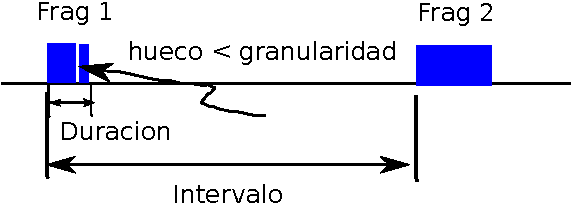
\includegraphics[width=4in]{figuras/intervalos-crop.pdf}  
  \caption{Definicion de intervalos}
  \label{fig:intervalos}
\end{figure}


Este segundo paso se tiene que hacer de manera automática con un
programa que tome las entradas siguientes:

\begin{itemize}
\item \textbf{Fichero de traza} en formato binario (trace.dat).
\item \textbf{PID del programa a sacar}, idealmente podría admitir una
  lista de PID's y generar una salida para cada uno.
\item \textbf{Instantes de comienzo y final del estudio} dados en
  tiempos relativos (milisegundos) a la traza capturada.
\item \textbf{Granularidad de ejecución} Hueco máximo de ejecución que
  se permite dentro de un fragmento para considerarlo ``un sólo bloque
  de ejecución''.  Esta granularidad se mide en microsegundos.
\end{itemize}

El programa generará para cada PID una tabla de la forma siguiente:

\begin{table}[h!]
  \centering
  \begin{tabular}{p{0.7in}|p{0.7in}|p{0.7in}|p{0.7in}|p{0.7in}|p{0.7in}}
    \textbf{Num Fragmento} & \textbf{Instante comienzo} &
    \textbf{Duracion} & \textbf{CPUs} & \textbf{Porcentage
      de relleno} & \textbf{Intervalo entre fragmento}\\ \hline
1 & 136.342 & 202.34 & 1 & 90 & 0 \\
2 & 1140.5523 & 206.34 & 1 & 95 & 1004 \\ 
3 & 2123.323 & 198.34 & 1 0 & 92 & 983\\
  \end{tabular}
  \caption{Tabla de salida del analizador de fragmentos}
  \label{tab:analisis}
\end{table}

Esta tabla deberá ser fácil de importar a hojas de cálculo (OO Calc,
Excel...) o entornos numéricos (Octave, Python Numpy, Matlab) para
realizar gráficos y estudios estadísicos con ella.

\subsection{Visualización de histograma y estadísticas}
\label{sec:estadistica}

Con los datos de la sección anterior se construiran (con hoja de
cálculo o programa similar) los datos siguientes:

\begin{enumerate}
\item Histograma de la distribución de duración de los fragmentos.
\item Histograma de la distribución de los intervalos entre
  fragmentos.
\item Histograma del porcentage de relleno.
\item Utilización de cada CPU
\item Media y desviación típica de duración de los intervalos y las
  separaciones.

\end{enumerate}

\subsection{Valoración de los resultados}
\label{sec:valoracion}

Con todos los datos (capturas de trace-cmd, visualización kernelshark,
tablas y estadísicas) se pide:

\begin{itemize}
\item Justificación de veracidad de los resultados calculados, es
  decir que las estadísticas son coherentes con las capturas.

\item Explicación de causas de desvíos respecto a posibles resultados
  iniciales.
\end{itemize}

% \bibliographystyle{abbrv}
% \bibliography{prac_linux_tools}



\end{document}

